\subsection{\FirstTimeDefine{\ProgramGraph}{\ProgramGraphEN}} 
\label{sec:sub:pg}

{\software} ถูกพัฒนาขึ้นมาเพื่อแก้ไขปัญหาในบริบทที่หลากหลาย ส่งผลให้มีโครงสร้างของ{\sourcecode}นั้นแตกต่างกันไปตามบริบทการพัฒนา
หรือปัญหาที่ต้องการแก้ไข ซึ่งไม่มีรูปแบบโครงสร้างที่คงตัว หากแต่ในขั้นตอนสร้างกรณีทดสอบนั้น\FirstTimeDefine{\tester}{\testerEN}
จำเป็นต้องทำความเข้าใจโครงสร้างของ{\software} ทั้งจากแผนภาพการออกแบบ เช่น แผนภาพยูเอ็มแอล (UML - Unified Modeling Language) 
และจาก{\sourcecode}โดยตรง ซึ่งการทำความเข้าใจโครงสร้างผ่าน{\sourcecode}โดยตรงนั้นย่อมสะท้อนลักษณะของ{\software}ที่เป็นปัจจุบันมากที่สุด
{\ProgramGraph} จึงเป็นวิธีการนำเสนอโครงสร้างที่ปรากฏอยู่ภายใน{\software} ณ ขณะที่สนใจ ช่วยให้{\tester}เข้าใจโครงสร้างของ{\software}
และออกแบบกรณีทดสอบได้มีประสิทธิภาพมากยิ่งขึ้น ซึ่งในงานวิจัยนี้จะนำ{\ProgramGraph}มาใช้ 2 ประเภท ด้วยกัน ได้แก่

\subsubsection{\FirstTimeDefine{\cfg}{\cfgen}}
\label{sec:sub:sub:cfg}

% หากกำหนดให้{\software} ด้วย\FirstTimeDefine{\DirectedGraph}{\DirectedGraphEN} 
หากแทน{\software} \code{P} แทนด้วยกราฟ \code{G} จะได้ว่า \code{G = (V, A)} เมื่อ \code{V (Vertex)} 
คือเซตของ{\Node}ในกราฟ ซึ่งแต่ละ{\Node}แทนแถวคำสั่งใน{\sourcecode} และ \code{A\ (Arcs)} 
คือเซตของคู่ลำดับโหนดที่มีความสัมพันธ์กันภายในกราฟซึ่งเชื่อมต่อกันแบบมีทิศทาง หาก \code{(v_m, v_n) \in A} จะหมายถึง 
"\Node\ \code{v_n} จะทำงานในลำดับถัดไปหลังจากที่ \code{v_m} ทำงานเสร็จสิ้น" \cite{Jorgensen2013} 
โดยที่ \code{v_i, v_j \in V} มีโหนดซึ่งไม่มีดีกรีเข้า \code{(d^+(v_i) = 0)} เป็นโหนดเริ่มต้น (Source node) 
และโหนดซึ่งไม่มีดีกรีออก \code{(d^-(v_j) = 0)} เป็นโหนดปลาย (Sink node) 
กล่าวได้ว่า{\cfg}นั้นถือว่าเป็นกราฟอวัฏจักรระบุทิศทาง (Directed acyclic graph: DAG) \cite{Bang-Jensen2009}\ 
ซึ่งรูปแบบความสำพันธ์ของกราฟโปรแกรมนั้น McCabe \cite{Watson1996} 
ได้เสนอรูปแบบโครงสร้างการทำงานขั้นพื้นฐานของการพัฒนาโปรแกรม (The primitive operations of structured programming) 
\figref{fig:graphtype}

\begin{figure}[ht!]
    \centering
    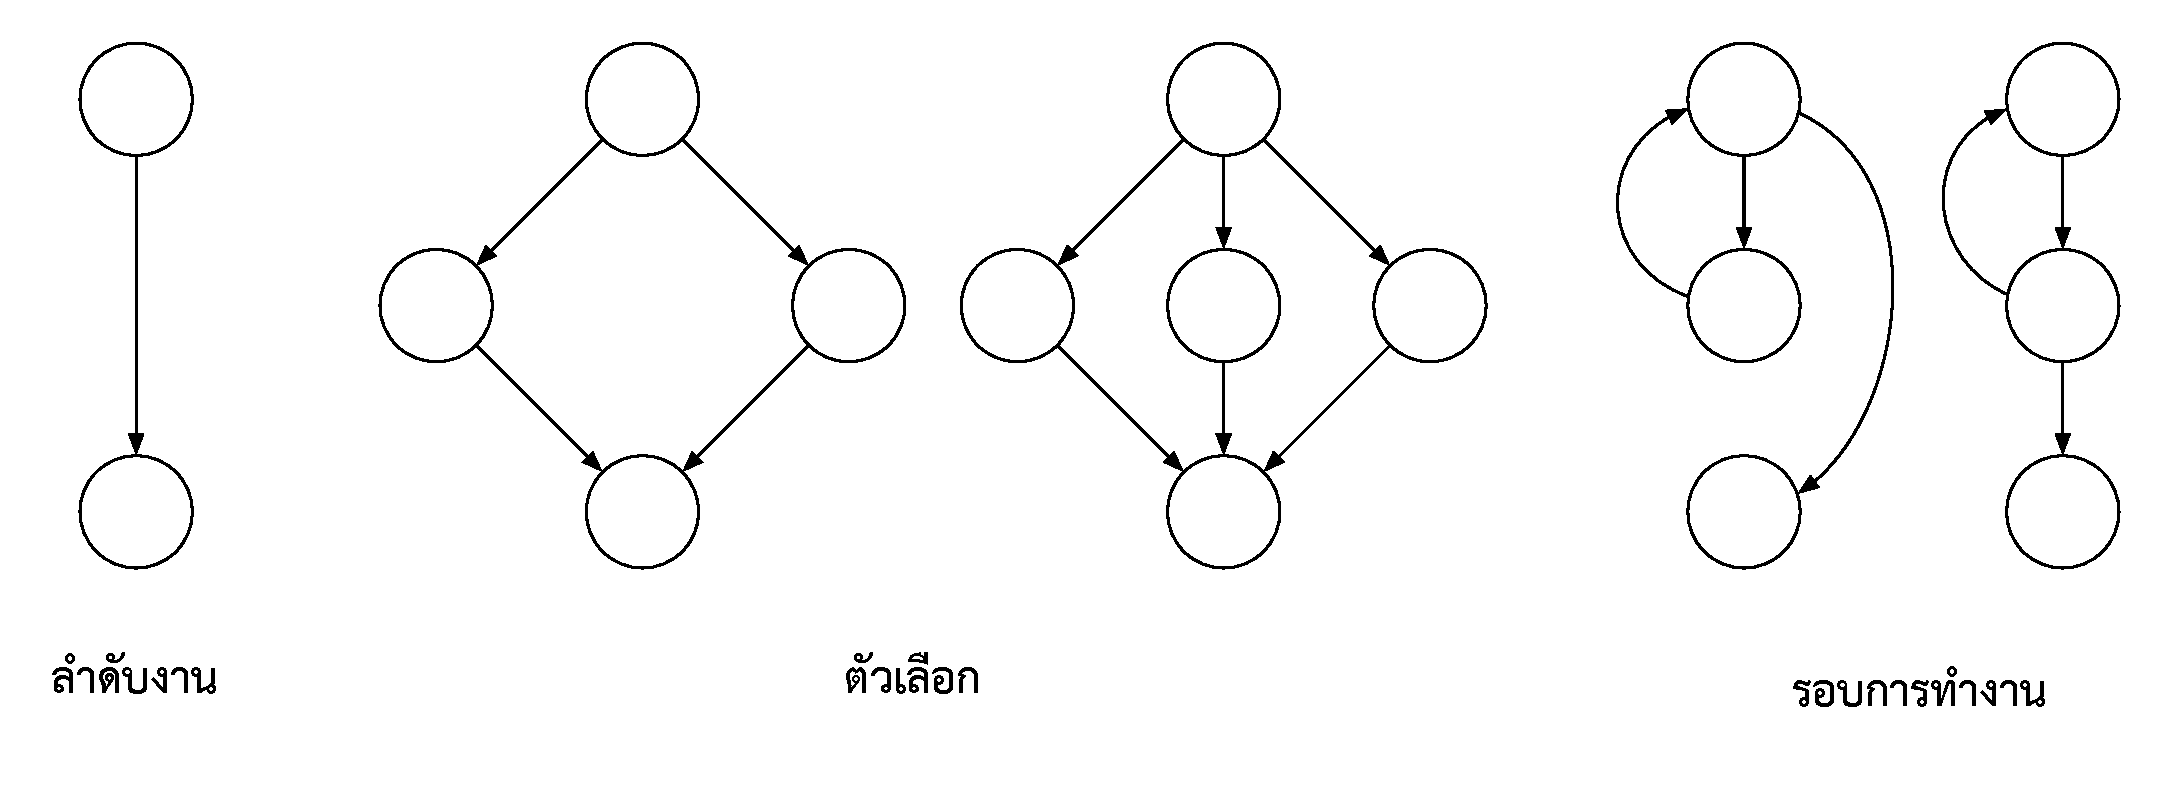
\includegraphics[width=0.9\textwidth]{graph-types}
    \caption{ประเภทของกราฟ}
    \label{fig:graphtype}
\end{figure}

จาก\figref{fig:pseudocodeGrading} เป็นรหัสเทียม (Psuedo code) ที่นำเสนอวิธีการคำนวณเกรดของนิสิตโดยรับข้อมูลคะแนน \code{(student\_score)} 
และคะแนนพิเศษ \code{(bonus\_score)} ของนิสิต หากมีคะแนนเป็น 0 จะได้เกรด \code{I}\ หากนิสิตได้คะแนนต่ำกว่า 80 คะแนน 
จะได้เกรด \code{U}\ หากมีคะแนนตั้งแต่ 80 ไปจนถึง 100 คะแนน นิสิตจะได้เกรด \code{S}\ ซึ่งจากชุดรหัสเทียมนี้ 
สามารถแปลงเป็นกราฟโปรแกรม เพื่อทำความเข้าใจโครงสร้างได้ดัง{\figref{fig:programGraph} 

\begin{figure}[ht!]
    \begin{algorithm}[H]
        \begin{algorithmic}[1]
            \STATE{Program {\bf "Simple Grading"}}
            \STATE{student\_score $\gets$ receive student score}
            \STATE{bonus\_score $\gets$ receive student's bonus score}

            \IF{bonus\_score > 0}
                \IF{student\_score <= 50} 
                    \STATE{student\_score = min(50, student\_score + bonus\_score)} 
                \ELSIF{student\_score <= 70} 
                    \STATE{student\_score = min(70, student\_score + bonus\_score)}
                \ENDIF
            \ENDIF

            \STATE{grade\_letter = ""}

            \IF{student\_score < 80} 
                \STATE{grade\_letter = 'U'} 
            \ELSIF{student\_score == 0}
                \STATE{grade\_letter = 'I'} 
            \ELSIF{student\_score <= 100}
                \STATE{grade\_letter = 'S'} 
            \ENDIF

            \STATE{print(grade\_letter)}
        \end{algorithmic}
    \end{algorithm}
    \caption{ชุดรหัสเทียมสำหรับคำนวณเกรดนิสิตจากคะแนนที่ได้รับ}
    \label{fig:pseudocodeGrading}
\end{figure}


\begin{figure}[ht!]
    \centering
    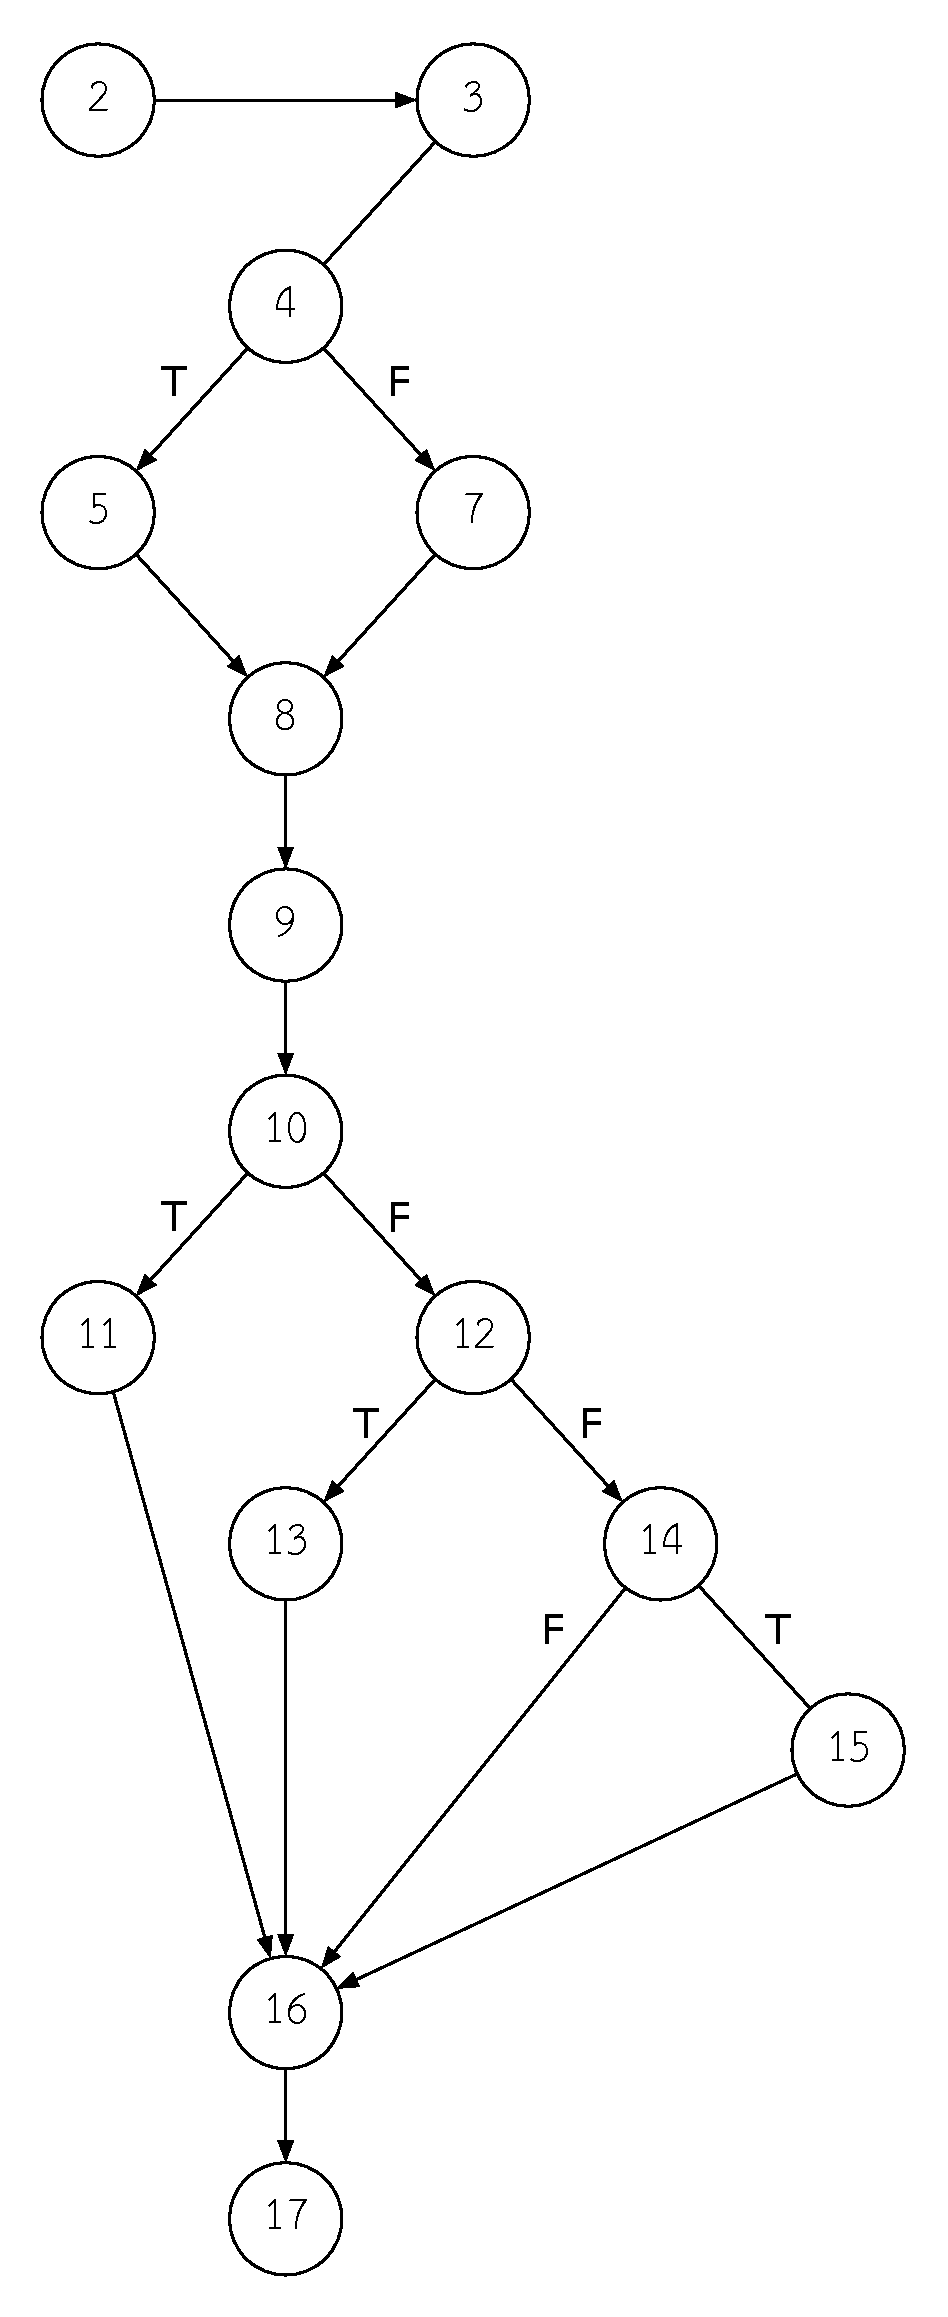
\includegraphics[height=0.80\textheight]{grading-program-graph}
    \caption{{\cfg}ของชุดรหัสเทียมสำหรับคำนวณเกรดนิสิต}
    \label{fig:programGraph}
\end{figure}

จาก{\figref{fig:programGraph}} เป็นการนำเสนอชุดรหัสเทียมจาก{\figref{fig:pseudocodeGrading} ในรูปของกราฟโปรแกรม 
โดยที่{\Node}ที่ 2, 3, 6, 8, 9, 10, 11, 13, 17, 18 และ 19 คือ{\Node}ที่แสดงถึงลำดับการดำเนินงาน 
และ{\Node} 4, 5, 6, 7, 12, 14 และ 16 เป็น{\FirstTimeDefine{\PredicateNode}{\PredicateNodeEN}} ภายในโปรแกรม 
โดยมีโหนด 2 และ 19 เป็น{\sourcenode} และ{\sinknode} ตามลำดับ 

จากโครงสร้าง{\sourcecode} ดัง{\figref{fig:pseudocodeGrading}} ทำให้เห็นได้ว่า {\tester}สามารถทำความเข้าใจโครงสร้างของ{\sourcecode} ได้ 
ถึงแม้{\tester}จะไม่มีประสบการณ์กับภาษาที่ใช้พัฒนา หากแต่{\tester}สามารวิเคราะห์หากรณีทดสอบได้จาก{\cfg}ข้างต้น 
ด้วยการพิจารณา{\PredicateNode}ที่ปรากฏบน{\FirstTimeDefine{\TestPath}{\TestPathEN}} ยกตัวอย่างเช่น 
หากเลือก{\Path}จาก{\figref{fig:programGraph}} เป็น{\TestPath}ดังที่แสดงใน{\figref{fig:testpath}} จะพบว่ามี{\PredicateNode}บน{\TestPath} 3 {\Node} 
ด้วยกัน นั่นคือ \code{4}, \code{5} และ \code{10} เมื่อพิจารณา{\PredicateNode}ทั้ง 3 {\Node}จะได้ข้อมูลทดสอบเป็น \code{bonus\_score = 1} และ 
\code{student\_score = 50} ซึ่งข้อมูลทดสอบที่สร้างขึ้นนี้สามารถทำให้โปรแกรมทำงานใน{\TestPath}ได้ 
ดังกรณีทดสอบใน\tabref{tab:simpleTestCase}

\clearpage
\begin{figure}[ht!]
    \centering
    \code{2\ - 3\ - (4)\ - (5)\ - 6\ - 10\ - 11\ - (12)\ - 13\ - 18 - 19}
    \caption{ตัวอย่าง{\TestPath}สำหรับโปรแกรมคำนวณเกรด}
    \label{fig:testpath}
\end{figure}


\begin{table}[ht!]
    \centering
    \caption{กรณีทดสอบ}
    \label{tab:simpleTestCase}
    \begin{tabular}{|l|c|c|c|}
        \hline
        \rowcolor{LightGray}
        Case ID     & bonus\_score  & student\_score    & Expected output \\
        \hline
        SC1         & 1             & 50                & U \\
        \hline
    \end{tabular}
\end{table}

\subsubsection{\FirstTimeDefine{\scg}{\scgEN}}

การพัฒนา{\software}เชิงวัตุ (Object-oriented programming: OOP) เป็นการรวมพฤติกรรม และความสามารถที่คล้ายคลึงกันเข้าไว้ด้วยกัน \cite{kindler2011}
ในลักษณะของ\FirstTimeDefine{\class}{\classEN} \FirstTimeDefine{\method}{\methodEN} และ \FirstTimeDefine{\attribute}{\attributeEN} 
ดังนั้นหากต้องทำเข้าใจถึงการมีปฏิสัมพันธ์ซึ่งกันและกันระหว่าง{\class}ภายในซอฟต์แวร์ภายใต้การทดสอบ (Software under test: SUT) จาก{\sourcecode} 
ที่ได้รับมานั้น{\scg}จึงเข้าช่วยแสดงความสัมพันธ์ในรูปแบบของ\FirstTimeDefine{\DirectedMultiGraph}{\DirectedMultiGraphEN}\ หากให้แทน{\software} \code{P} 
แทนด้วยกราฟ \code{G} จึงสามารถเขียนความสัมพันธ์ในรูปของทูเปิ้ล 6 รายการ \code{G = (V, E, tail, head, \ell_V, \ell_E, \sigma, \delta)}

\begin{table}[ht!]
    \begin{tabular}{ll}
        เมื่อ & \code{V} คือ เซตซึ่งมีสมาชิกจำกัดซึ่งเป็น{\Node}ภายในกราฟ \\
            & \code{E} คือ เซตซึ่งมีสมาชิกจำกัดของ{\Edge} \\
            & \code{tail:E \rightarrow V} คือ ฟังก์ชันซึ่งกำหนด{\Edge}ให้กับ{\Node}หาง (tail) \\
            & \code{head:E \rightarrow V} คือ ฟังก์ชันซึ่งกำหนด{\Edge}ให้กับ{\Node}หัว (head) \\
            & \code{\ell_V:V \rightarrow tail} คือ ฟังก์ชันที่กำหนดแผ่นป้ายให้กับ{\Node} \\
            & \code{\ell_E:E \rightarrow head} คือ ฟังก์ชันที่กำหนดแผ่นป้ายให้กับ{\Edge} \\
    \end{tabular}
\end{table}

\begin{figure}[ht!]
    \lstset{basicstyle=\small,style=thesiscodestyle,language=java}
    \lstinputlisting[language=Java]{related/SimpleQuiz.java}
    \caption{{\sourcecode}ภาษาจาวาสำหรับอ่านคะแนนคำถามภายในชั้นเรียน}
    \label{fig:javaQuiz}
\end{figure}

\begin{figure}[ht!]
    \lstset{basicstyle=\small,style=thesiscodestyle,language=java}
    \lstinputlisting[language=Java]{related/SimpleBonusScore.java}
    \caption{{\sourcecode}ภาษาจาวาสำหรับคำนวนคะแนนเพิ่มพิเศษ}
    \label{fig:javaBonusScore}
\end{figure}

\begin{figure}[ht!]
    \lstset{basicstyle=\small,style=thesiscodestyle}
    \lstinputlisting[language=Java]{related/SimpleGrading.java}
    \caption{{\sourcecode}ภาษาจาวาสำหรับคำนวณเกรดนิสิต}
    \label{fig:javaGrading}
\end{figure}

หาก{\class} \code{SimpleQuiz}, \code{SimpleBonusScore} และ \code{SimpleGrading} ดังแสดงใน 
\figref{fig:javaQuiz}, \ref{fig:javaBonusScore} และ \ref{fig:javaGrading} แทนด้วย \code{Q}, \code{B} และ \code{G} ตามลำดับ
จะสามารถสร้าง{\scg}เพื่ออธิบายความสัมพันธ์ของ{\class}ทั้ง 3 นี้ได้ดัง \figref{fig:scggrading} 
โดยมี{\method}ต้นทางที่เรียกใช้งานและ{\method}ปลายทางที่ถูกเรียกใช้ เป็นป้ายกำกับ

\begin{figure}[htb!]
    \centering
    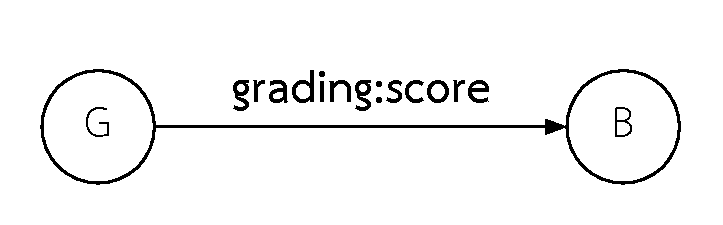
\includegraphics[width=0.8\textwidth]{simple-static-call-graph}
    \caption{{\scg}โปรแกรมคำนวณเกรดนิสิต}
    \label{fig:scggrading}
\end{figure}

% - - - - - - - - - - - - - - - - - - - -
\subsection{\FirstTimeDefine{\InfeasiblePath}{\InfeasiblePathEN}}

\InfeasiblePath คือ ทางเดินที่ไม่สามารถหาค่าทุก ๆ ความเป็นไปได้ซึ่งสอดคล้องกับ{\PredicateNode}ที่อยู่บนทางเดินนั้น 
เพื่อทำให้โปรแกรมทำงานบนเส้นทางนั้นได้ \cite{Naik2008} หากพิจารณาจากชุดรหัสเทียมใน{\figref{fig:pseudocodeGrading}} 
และกราฟใน{\figref{fig:programGraph}} ประกอบเข้าด้วยกัน จะพบว่าทางเดิน 
\code{\overline{12}\ \textendash\ 14\ \textendash\ 15 \textendash\ 18 \textendash\ 19} คือ {\bf \InfeasiblePath} 
ดังแสดงใน{\figref{fig:infeasiblePath}} เนื่องจากไม่สามารถหาค่าที่สอดคล้อง กับ\PredicateNode\ 12 และ 14 
นั่นคือ \code{student\_score \geq 80} และ \code{student\_score = 0} ได้ในทุก ๆ กรณี

\begin{figure}[t!]
    \centering
    \includegraphics[width=0.5\textwidth]{grading-program-graph-subgraph}
    \caption{โครงสร้างของโปรแกรมที่พบ{\InfeasiblePath}}
    \label{fig:infeasiblePath}
\end{figure}


ดังนั้นการทดสอบโปรแกรมนั้นจึงจำเป็นจะต้องวิเคราะห์{\InfeasiblePath}ที่อยู่ภายในโครงสร้างของโปรแกรมเพื่อรายงานผลให้นักพัฒนาได้ทราบและแก้ไข
ต่อไปได้

% \subsection{\FirstTimeDefine{\Cyclomatic}{\CyclomaticEN}}
% 
% ในการวัดความซับซ้อนเชิงโครงสร้างของโปรแกรมนั้น McCabe ได้กำหนด \Cyclomatic\ \cite{McCabe1976}\ 
% ไว้เพื่อเป็นมาตรวัดความซับซ้อนของโปรแกรม โดยใช้การพิจารณาจากจำนวน\Node\ \Edge และ\PredicateNode\ ที่ประกอบกันภายใน\ProgramGraph\ 
% ดัง\eq{eq:complexitymeasureStronglyConnected} และ \eq{eq:complexitymeasure}
% 
% \begin{align}
%     v(G) &= e - n + p \label{eq:complexitymeasureStronglyConnected} \\
%     v(G) &= e - n + 2p \label{eq:complexitymeasure} 
% \end{align}
% 
% \begin{table}[ht!]
%     \begin{tabular}{lcl}
%     เมื่อ & $v(G)$    & คือ ค่า{\Cyclomatic}ที่คำนวณได้               \\
%         & $e$       & คือ จำนวน{\Edge}ใน\ProgramGraph            \\
%         & $n$       & คือ จำนวน{\Node}ใน\ProgramGraph            \\
%         & $p$       & คือ จำนวนพื้นที่ที่เชื่อมต่อกันใน\ProgramGraph   \\
%     \end{tabular}
% \end{table}
% 
% โดยที่ \eq{eq:complexitymeasureStronglyConnected} จะใช้กับกราฟที่เชื่อมต่อกันแบบเข้ม (Strongly connected graph) 
% นั่นคือกราฟนั้นจะต้องมีทางเดินจาก $n_j$ ไปยัง $n_k$ เสมอ แต่หากไม่ใช่แล้วจะใช้ \eq{eq:complexitymeasure} โดยจะกำหนดให้ 
% $p = 1$ จาก{\ProgramGraph}ใน{\figref{fig:programGraph}} ซึ่งมี{\Edge}ทั้งสิ้น 23 เส้น และจำนวน{\Node}ทั้งสิ้น 
% 18 \Node\ ดังนั้นหากคำนวนระดับความซับซ้อนตาม{\Cyclomatic}ของ{\ProgramGraph}นี้ จะได้ว่า
% 
% \begin{align*}
%     v(G) &= e - n + 2p \\
%          &= 23 - 18 + 2 \\
%     v(G) &= 7 
% \end{align*}
% 
% จากคำของ McCabe แล้วโปรแกรมไม่ควรมีค่า{\Cyclomatic}มากกว่า 15 โดยที่ค่าความซับซ้อนที่แนะนำอยู่ที่ 10 \cite{McCabe1976}
